\begin{center}
    \section*{\fontsize{20}{20}\selectfont Chapter 3}
\end{center}
\vspace{10mm}
\section{Research Methodology}

This chapter explains how we built the potato leaf disease detection and advice system, step by step. We follow the report format. First we give the full framework. Then we describe the dataset and the project requirements, including data collection, preprocessing and how the CNN selects features. After that we explain the three models (Custom Lightweight CNN, ResNet50 and MobileNetV2). Finally we explain the Grad-CAM module and the Gemini LLM advice module.

\subsection{Proposed Framework}
The system has four stages. It classifies the image, shows why it made the decision and gives safe advice in normal language. Figure~\ref{fig:workflow} shows the stages:
\begin{enumerate}
    \item \textbf{Data loading and preprocessing.} Field images from the 7-class dataset are split with stratified sampling ($80:10:10$) and resized to $224 \times 224 \times 3$. Training images are augmented on the fly. Each model then gets its own type of normalization.
    \item \textbf{Classification with deep learning.} We train and test three CNN models with the same loss and the same metrics: our Custom Lightweight CNN, a frozen ResNet50 benchmark and a MobileNetV2 benchmark trained from scratch.
    \item \textbf{Checking with Grad-CAM.} Gradient-weighted Class Activation Mapping (Grad-CAM) looks at the last convolutional layer. It shows whether the prediction comes from the real leaf lesions or from the background.
    \item \textbf{LLM advice based on confidence.} The predicted disease and the softmax confidence are sent to Google Gemini (\texttt{gemini-3.1-flash-lite}) with strict safety rules. Gemini writes a simple summary of the symptoms, management steps and a warning when the confidence is low.
\end{enumerate}

\begin{figure}[htbp]
\centering
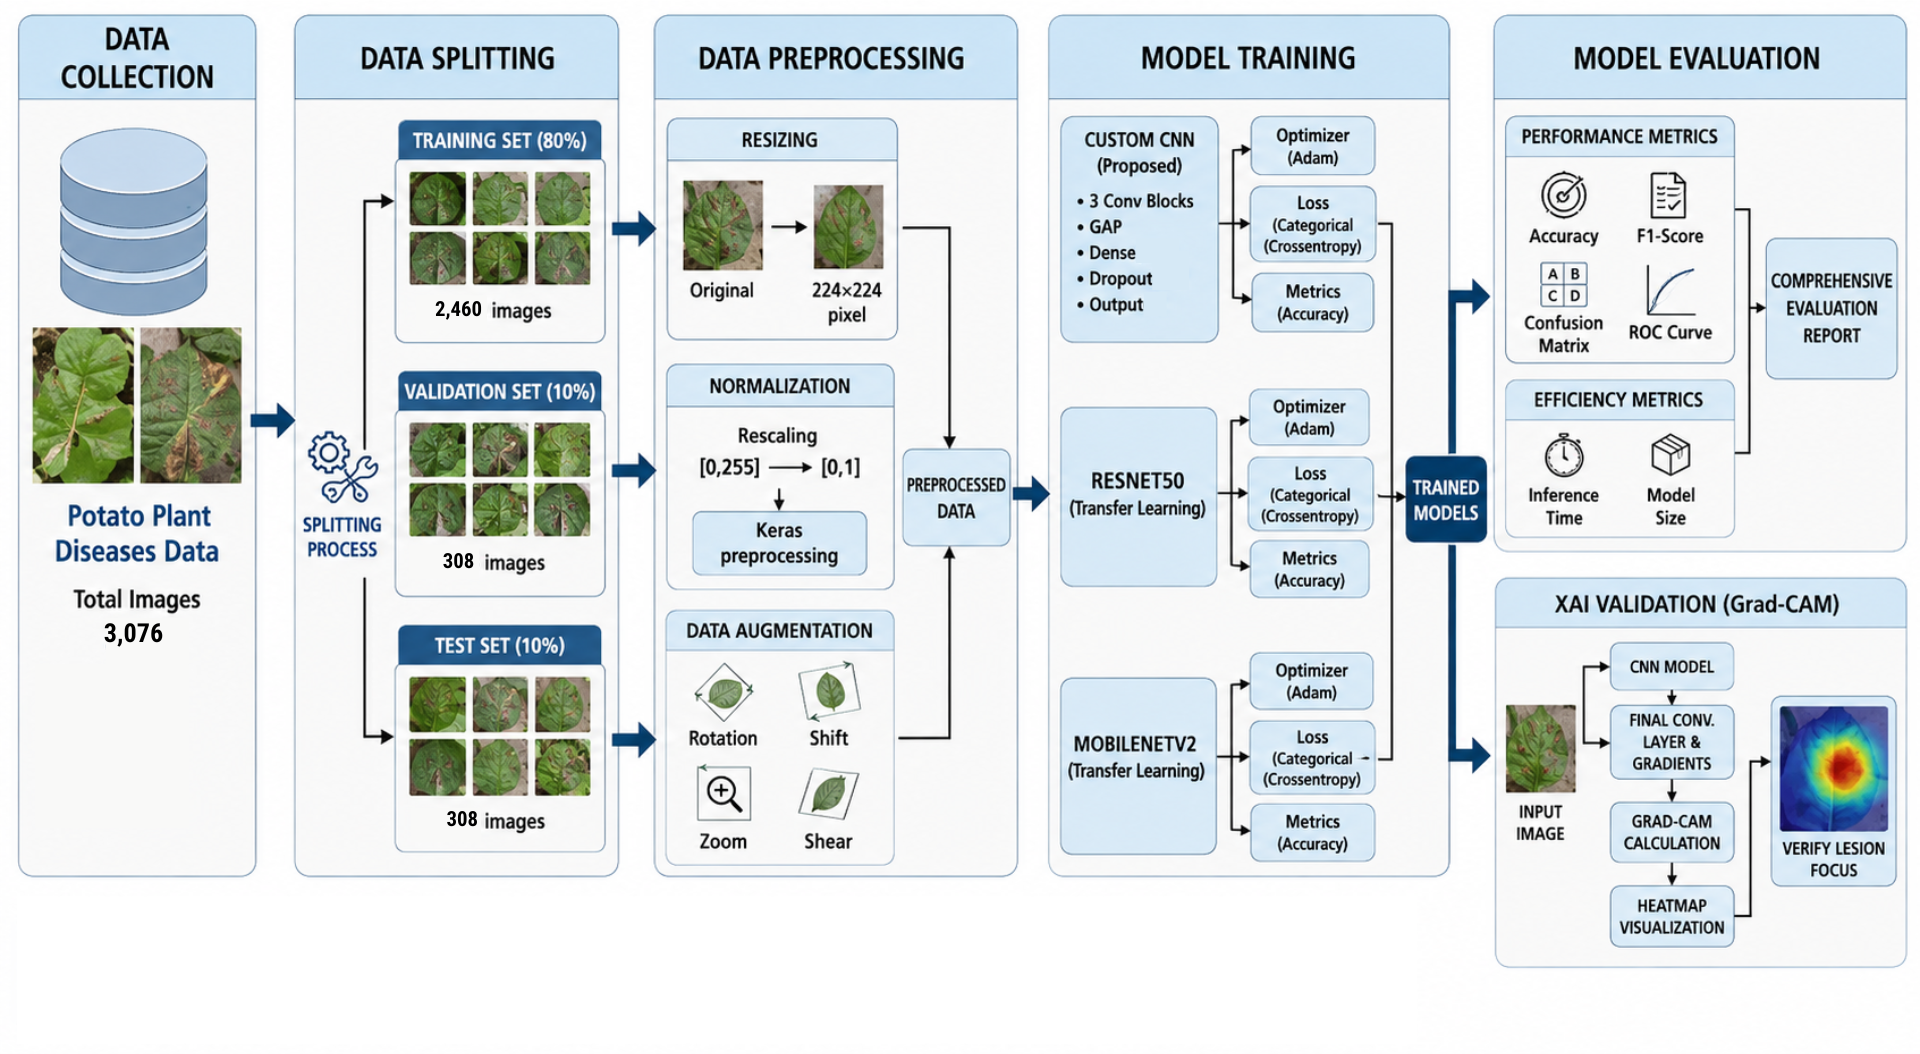
\includegraphics[width=0.95\textwidth]{image/docx_image2.png}
\caption{Workflow Diagram (Block Diagram of Proposed Methodology).}
\label{fig:workflow}
\end{figure}

Before the full build, we checked whether the framework was feasible in three ways.

\textit{Technical.} The pipeline uses well-known open-source Python libraries, mainly TensorFlow~2.20 and Keras \cite{abadi2016tensorflow}, in Kaggle cloud notebooks. Kaggle offers GPUs, but in the reported baseline run CUDA did not start (\texttt{failed call to cuInit}), so the code ran on the CPU. The CPU was enough to test the whole pipeline from start to end, but it limited how many epochs we could train.

\textit{Operational.} After training, the system is easy to use. The user uploads a leaf photo and gets the predicted disease, the confidence, a Grad-CAM heatmap and advice from the LLM. Farmers and agricultural extension workers can use it without special skills.

\textit{Economic.} All the main software (Python, TensorFlow, Scikit-learn, OpenCV, Jupyter and Kaggle Notebooks) is free and open source. The small custom model needs little hardware to run. The Gemini API is called only once per diagnosis, so the cost of the advice stays low.

\subsection{Dataset Analysis and Project Requirements}
We use the \textit{Potato Leaf Disease Dataset in Uncontrolled Environment} from Shabrina et al.\ \cite{shabrina2024novel}, which is available on Kaggle. Lab datasets such as PlantVillage \cite{hughes2015open} have plain backgrounds. This dataset is different. It has 3,076 color photos taken in the field, with soil, plastic mulch, hands, shadows and other leaves in the background. There are seven classes: six disease or pest classes and one healthy class. (\textit{Phytopthora} is the folder name used in the Kaggle dataset for \textit{Phytophthora} late blight, and we kept that spelling.)

Table~\ref{tab:class_dist} shows that the classes are very uneven. The largest class (\textit{Fungi}, 748 images) is about 11 times bigger than the smallest class (\textit{Nematode}, 68 images). The \textit{Healthy} class is also small (201 images). We had to handle this when splitting and testing the data. Otherwise a model could get a low loss just by predicting the large classes, and the result would be misleading.

\begin{table}[htbp]
\caption{Dataset Classes and Distribution of the Potato Leaf Disease Dataset}
\label{tab:class_dist}
\begin{center}
\begin{tabularx}{0.9\textwidth}{| X | X | c | c |}
\hline
\textbf{Plant Name} & \textbf{Disease / Health Status} & \textbf{Number of Images} & \textbf{Share (\%)} \\
\hline
Potato & Fungi & 748 & 24.32\% \\
\hline
Potato & Pest & 611 & 19.86\% \\
\hline
Potato & Bacteria & 569 & 18.50\% \\
\hline
Potato & Virus & 532 & 17.30\% \\
\hline
Potato & Phytopthora & 347 & 11.28\% \\
\hline
Potato & Healthy & 201 & 6.53\% \\
\hline
Potato & Nematode & 68 & 2.21\% \\
\hline
\textbf{Total Images} & \textbf{7 Classes} & \textbf{3,076} & \textbf{100.00\%} \\
\hline
\end{tabularx}
\end{center}
\end{table}

\subsubsection{Data Collection and Preprocessing}
We listed the image file paths and their folder labels in a Pandas DataFrame. We then split them with stratified sampling (\texttt{random\_state = 42}) at $80:10:10$ into training (2,460 images), validation (308 images) and unseen test (308 images) sets. This keeps the same share of each class in all three sets.

Before the images go into the networks, we apply three preprocessing steps.

\textit{Resizing.} The field photos have different sizes. We resize all of them to $224 \times 224 \times 3$ with \texttt{flow\_from\_dataframe}.

\textit{Normalization for each model.} For the Custom CNN (Path~A), we divide the pixel values by $255.0$, so they go from $[0, 255]$ to $[0, 1]$. For ResNet50 and MobileNetV2 (Path~B), we use the Keras \texttt{preprocess\_input} function of each model. For ResNet50 this changes the channel order and subtracts the ImageNet mean. For MobileNetV2 it scales the values to $[-1, 1]$.

\textit{Augmentation during training.} To reduce overfitting and to handle leaves facing different ways, the training generator applies random rotation (up to $20^\circ$), width and height shifts (up to 20\%), random zoom (up to 20\%, filling with the nearest pixel) and horizontal flips \cite{shorten2019survey}.

\subsubsection{Feature Selection and Representation}
Classic plant disease pipelines pick features by hand. They use descriptors such as color histograms, Gray-Level Co-occurrence Matrix (GLCM) texture or Scale-Invariant Feature Transform (SIFT) keypoints \cite{alhiary2011fast, arivazhagan2013detection, pujari2016image}. In field photos with soil, plastic mulch, shadows and fingers, these simple features often cannot separate the background from small lesions on the leaf \cite{ngugi2021recent}.

In our pipeline the convolutional layers choose the features themselves, step by step.

\textit{Convolution at several scales.} The first $3 \times 3$ convolution layers pick up small edges, color contrast and spots. The deeper blocks combine these into larger lesion textures and leaf shapes.

\textit{Activation and normalization.} Batch Normalization \cite{ioffe2015batch} keeps the values inside the network stable from batch to batch. Swish activation ($f(x) = x \cdot \sigma(\beta x)$) \cite{ramachandran2017swish} keeps a small, smooth gradient for negative inputs, so more information passes through than with ReLU, which cuts negative values to zero.

\textit{Compression with Global Average Pooling (GAP).} We could flatten the last $28 \times 28 \times 128$ tensor into $100{,}352$ numbers, but this would add a huge number of parameters and cause overfitting. Instead, GAP takes the average of each of the 128 channels, which gives a vector of only $128$ values. These values keep the channel information that separates the classes. They feed the dense classifier, and the same feature map is used for Grad-CAM.

\subsubsection{Software and Hardware Project Requirements}
We set the following requirements so the work can be repeated.

\textit{Functional requirements.} The system must (i) accept normal RGB leaf images (JPG, PNG); (ii) resize and normalize each input for the chosen model; (iii) output one of the 7 potato classes with its softmax confidence; (iv) draw a Grad-CAM heatmap on the leaf to show the important regions \cite{selvaraju2017grad}; and (v) write advice for farmers through Gemini, with a clear warning when the confidence is low.

\textit{Non-functional requirements.} The target is more than 95\% test accuracy for real use, fast inference (best under 100~ms per image for interactive use) and a modular design so new disease classes can be added later.

\textit{Dataset requirements.} 3,076 labeled RGB field images in the 7 classes of the Kaggle potato dataset taken in uncontrolled conditions \cite{shabrina2024novel}.

\textit{Hardware requirements (training and use).} For training, we planned a multi-core x86 CPU (Intel Core~i5, Ryzen~5 or a cloud vCPU), at least 16~GB RAM and an NVIDIA GPU with at least 12~GB VRAM for fast training. For use after training, a normal phone or laptop CPU with at least 4~GB RAM should be enough to run the small model.

\subsection{Algorithm and Model Analysis}

\subsubsection{Proposed Custom Lightweight CNN}
We designed the Custom Lightweight CNN to have as few parameters and as little memory use as possible, while it can still learn features layer by layer.

\textit{Input layer.} It takes normalized RGB images of shape $(224, 224, 3)$.

\textit{Convolution blocks.} There are three feature blocks, one after another. Each block has two $3 \times 3$ \texttt{Conv2D} layers. The number of filters grows from block to block ($16 \rightarrow 32$, $32 \rightarrow 64$ and $64 \rightarrow 128$). Each block also has \texttt{BatchNormalization} \cite{ioffe2015batch}, Swish activation \cite{ramachandran2017swish}, $2 \times 2$ \texttt{MaxPooling2D} and \texttt{Dropout} ($0.20$, $0.20$ and $0.25$) \cite{srivastava2014dropout}.

\textit{Small classifier head.} A \texttt{GlobalAveragePooling2D} layer turns the $(28, 28, 128)$ feature map into 128 values. Then come a 128-unit \texttt{Dense} layer, \texttt{BatchNormalization}, Swish, \texttt{Dropout(0.40)} and a 7-unit \texttt{Softmax} output layer. The network has 162,887 parameters in total (161,959 trainable). The raw weights take 636.28~KB, and the saved file is 1.98~MB.

\subsubsection{ResNet50 Architecture}
ResNet50 \cite{he2016deep} is our deep benchmark model. It uses identity skip connections so the gradients do not vanish across its 50 layers. We removed its top classification layers (\texttt{include\_top = False}) and added a small head (\texttt{GlobalAveragePooling2D}, \texttt{Dense(64)}, \texttt{BatchNormalization}, Swish, \texttt{Dropout(0.30)} and a 7-class \texttt{Softmax}). The ImageNet weights could not be downloaded in the offline Kaggle session. So the backbone started with random weights (\texttt{weights = None}) and was kept frozen (\texttt{trainable = False}). Only the 131,719 head parameters were trainable, out of 23,719,559 in total (90.48~MB). This means the test measures fixed random convolution filters, not real ImageNet transfer learning.

\subsubsection{MobileNetV2 Architecture}
MobileNetV2 \cite{sandler2018mobilenetv2, howard2017mobilenets} is the usual efficient model for phones. It uses depthwise separable convolutions with inverted residual bottlenecks to need fewer operations (FLOPs). We added the same kind of custom head to the backbone with \texttt{include\_top = False} (2,340,679 parameters in total, 2,306,439 trainable). We had no ImageNet weights here either, so we used \texttt{weights = None} and set all backbone layers to \texttt{trainable = True}. The model therefore tried to learn all its filters from zero on the 2,460 training images.

\subsubsection{Training Optimization and Evaluation Protocol}
All three models use the Adam optimizer (starting learning rate $0.001$) and Categorical Cross-Entropy loss with label smoothing ($\epsilon = 0.1$), which stops the model from being too confident. During training we used three callbacks: \texttt{ModelCheckpoint} (it saves the weights with the best validation loss in \texttt{.keras} format), \texttt{EarlyStopping} and \texttt{ReduceLROnPlateau}. On the 308 unseen test images we measured accuracy, test loss, precision, recall, F1-score, confusion matrices, micro-average ROC-AUC, CPU inference time (ms per image) and the size of the saved file (MB) \cite{grandini2020metrics}.

\subsection{Explanation of Different Modules}

\subsubsection{Explainable AI Module (Grad-CAM)}
We want to see what the CNN is looking at, and make sure it does not rely on the background. For this we added Gradient-weighted Class Activation Mapping (Grad-CAM) \cite{selvaraju2017grad} on the last convolutional layer (\texttt{conv2d\_5}). Let $A^k \in \mathbb{R}^{u \times v}$ be the $k$-th feature map of this layer, and let $y^c$ be the score of the predicted class $c$ before softmax. The weight $\alpha_k^c$ of each channel is the average of the class gradients over all positions $(i, j)$:
\begin{equation}
\alpha_k^c = \frac{1}{Z} \sum_{i} \sum_{j} \frac{\partial y^c}{\partial A_{ij}^k},
\end{equation}
where $Z = u \times v$. We add up the feature maps using these weights and apply a Rectified Linear Unit ($\text{ReLU}$). This gives a rough heatmap that keeps only the features that support class $c$:
\begin{equation}
L_{\text{Grad-CAM}}^c = \text{ReLU}\!\left(\sum_{k} \alpha_k^c A^k\right).
\end{equation}
We normalize the heatmap, resize it to $224 \times 224$ and blend it onto the original leaf photo. A person can then check whether the model looks at the visible lesions or at something wrong in the background.

\subsubsection{LLM-Based Advisory Module}
A class name alone does not tell a farmer what to do in the field. So we connect the CNN output to a Large Language Model (Google Gemini, model \texttt{gemini-3.1-flash-lite}) through the official \texttt{google-genai} Python SDK \cite{google2026gemini}. The module works as follows.

\textit{What is sent to the LLM.} Only the name of the predicted disease and the softmax confidence are put into the prompt. This is true in the notebook (through \texttt{get\_llm\_disease\_advice()} and \texttt{predict\_and\_explain()}) and in the web backend. The leaf photos are not sent to the outside API.

\textit{Structured advice and chat.} The module writes a short disease brief with the parts \textit{Overview}, \textit{Symptoms}, \textit{Possible Causes}, \textit{Recommended Actions} and \textit{Prevention}. Farmers can also ask follow-up questions in Bengali or English about their own leaf.

\textit{Safety rules and the API key.} The system prompt does not allow made-up pesticide brand names or chemical doses. It tells the model to point the farmer to product labels, local agricultural extension services or crop advisors, and never to claim 100\% certainty. When the model's confidence is low, a clear warning asks the farmer to check the result. The API key is stored in environment secrets (Kaggle Secrets or server environment variables), not written in the source code.

\subsubsection{Web Application Module}
To make the diagnosis, explanation and advice usable outside the research notebook, we put all parts together in a full-stack web application (\url{https://potato.mamunlab.com/}). The \textbf{FastAPI} backend handles image preprocessing, Keras model inference, Grad-CAM heatmaps, PDF/CSV reports and calls to the Gemini API. The \textbf{React} frontend adapts to phone screens. The app works in \textbf{English and Bengali}, can switch between \textbf{Light and Dark themes}, and always shows a safety note (\textit{``AI-based preliminary classification---not a definitive diagnosis''}). It has five main views:
\begin{itemize}
    \item \textbf{Detect:} takes one potato leaf photo by drag and drop, file upload (JPG/PNG up to 10~MB) or the camera (\textit{Take a photo}) for use in the field.
    \item \textbf{Results:} shows the predicted condition, the confidence, the probabilities of the top classes (with a \textit{Show all classes} switch) and the original photo next to the Grad-CAM \textit{Attention overlay}. It also has an experimental attention-level indicator, which is clearly labeled as an estimate and not a tested severity score. Buttons open the AI chat, show the disease information or download a \textbf{PDF report}.
    \item \textbf{Batch Analysis:} checks up to 12 leaf photos at once (without Grad-CAM, to be faster). It counts Healthy and Diseased leaves, lists the prediction, confidence and top-3 class probabilities for each photo and exports the table with \textbf{Download CSV}.
    \item \textbf{Chat (Disease Assistant):} starts a Gemini conversation with the predicted class and confidence already filled in. Farmers can ask more questions in English or Bengali, and the safety notes are always added.
    \item \textbf{Info (Disease Information):} shows AI-written reference cards for the disease (\textit{Overview}, \textit{Symptoms}, \textit{Possible causes}, \textit{Recommended actions} and \textit{Prevention}), with a link to the AI assistant.
\end{itemize}

\clearpage
